\section{API}

\subsection{Desarrollo del API}

Para el desarrollo del API se utiliza el paquete sphinx de Python \url{http://www.sphinx-doc.org} y el tema Read The Docs \url{https://readthedocs.org}.

La selección de estas herramienta se debe a que permite generar documentación automáticamente a través de comentarios en el código, lo que facilita en gran medida esta tarea

\subsection{Ejemplos del API}

La pagina inicial de la librería puede verse en la figura  \ref{fig:lamfriaA}

\begin{figure}[H]
    \centering
    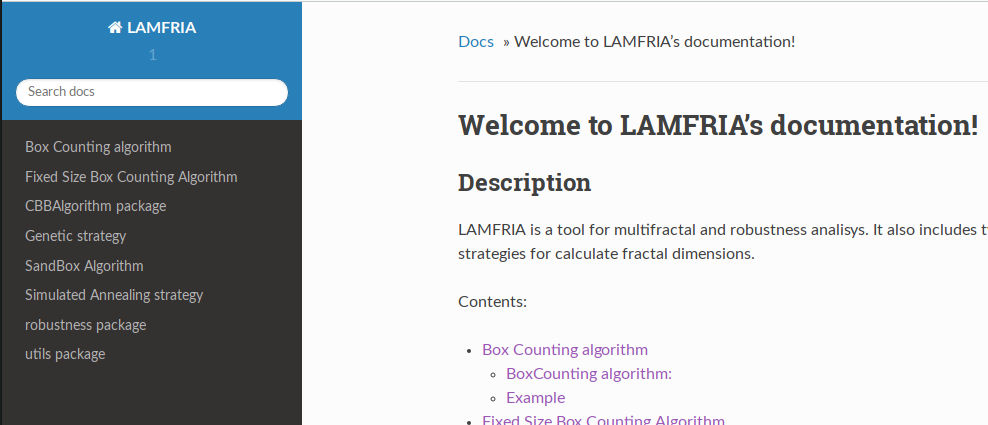
\includegraphics[scale=0.5]{Capitulo7Libreria/imagenes/lamfriaA.png}
    \caption{Pagína inicial del API}
    \label{fig:lamfriaA}
\end{figure}